\documentclass{article}
\usepackage{textcomp}
\usepackage[english]{babel}
\usepackage[utf8]{inputenc}
\usepackage{lmodern}
\usepackage{textcomp}
\usepackage[T1]{fontenc}
\usepackage{ucs}
\usepackage{amssymb}
\usepackage{amsmath}
\usepackage{courier}
\usepackage{graphicx}
\usepackage{a4wide}

\newcommand{\quality}[1]{q_{#1}}
\newcommand{\minfun}{\text{min}}
\newcommand{\realvec}[1]{\mathbf{#1}}
\newcommand{\norm}[1]{\left\| #1 \right\|}
\newcommand{\derivative}[2]{\frac{\partial #1}{\partial #2}}
\newcommand{\timederivative}[1]{\derivative{#1}{t}}
\newcommand{\realnumber}{\mathbb{R}}
\setcounter{secnumdepth}{2}




% Style used for devices.
\newcommand{\device}[1]{\texttt{#1}}

% Words to denote the devices that we are talking about
\newcommand{\anemobox}{\device{anemobox}}
\newcommand{\phone}{\device{phone}}
\newcommand{\anemolab}{\texttt{anemolab}}

% Abbreviations for the above words
\newcommand{\abbrbox}{\device{[B]}}
\newcommand{\abbrphone}{\device{[P]}}
\newcommand{\abbrlab}{\device{[L]}}


\author{Jonas Östlund\\jonas@anemomind.com}
\date{\today}
\title{Anemomind Nividic Data Transfer Architecture}

\begin{document}
\maketitle
\section{Introduction}
The purpose of this document is to outline the architecture for transferring data between the different devices involved with the Nividic product. Specifically, there are three types of devices: an \anemobox{}, a mobile \phone{} or tablet, and \anemolab{}. We also outline a high-level description of the protocol used to communicate between the devices.

\section{Requirements}
The architecture should at least accomodate the following operations that will be necessary for Nividic:
\begin{itemize}
  \item Move log files from \anemobox{} to \anemolab{}
  \item Move photos and notes from \phone{} to \anemolab{}
  \item Move calibration parameters from \anemolab{} to \anemobox{}
\end{itemize}
but should be general enough to allow for other type of data transfer too in later product releases.

Different architectures and protocols are defined for different requirements, constraints and use cases. For instance, the TCP/IP suite is designed for robust delivery of data over the internet, whereas the UDP protocol is designed for low latency. The architecture and high-level outline of the protocol in this document is designed according to the following assumptions and considerations:
\begin{itemize}
  \item \textbf{Storage capacity} on any device \textbf{is abundant}. For instance, there are Micro SD cards that can store thousands of photos or several weeks of boat logs. Such cards can be on both the \anemobox{} and \phone{}. Cloud storage for \anemolab{} is also abundant. Therefore, we assume that there is no need to delete data prematurely, before we are absolutely sure that it has reached its destination.
  \item \textbf{Communication links} between two devices \textbf{rarely exist}. For instance, a sailor may be sailing mostly in his week-end but spend the rest of the week working. Therefore, there will only be a communication link (e.g. bluetooth) between his mobile phone and the boat in the week-end when he is sailing, but not when he is away from his boat with the phone in his pocket. Likewise, it may not be possible to always establish a communication link between the mobile phone and the internet if he is sailing far away from the coast or along the coast of a foreign country where data traffic is limited. 
  \item \textbf{Robustness over latency.} The information that is transferred between devices can be very valuable, not the least in terms of time and effort. For instance, a log file containing hours of recorded data correspond to the same amount of time of real sailing, maybe in tough and cold conditions. Such recordings must not be lost when they are transferred. It is usually more important that the transfer is robust than slightly reducing the time the user has to wait for some operation. We thus adopt a policy of eagerly trying to propagate data from one device to another device in order to maximize the chance that the data will eventually reach its destination.
\end{itemize}

For the Nividic release, we assume that there will be communication links between \anemobox{} and \phone{} (such as bluetooth), and between \phone{} and \anemolab{} (e.g. with TCP/IP), as illustrated in Fig.~\ref{fig:arch}.
\begin{figure}
\begin{tabular}{cc}
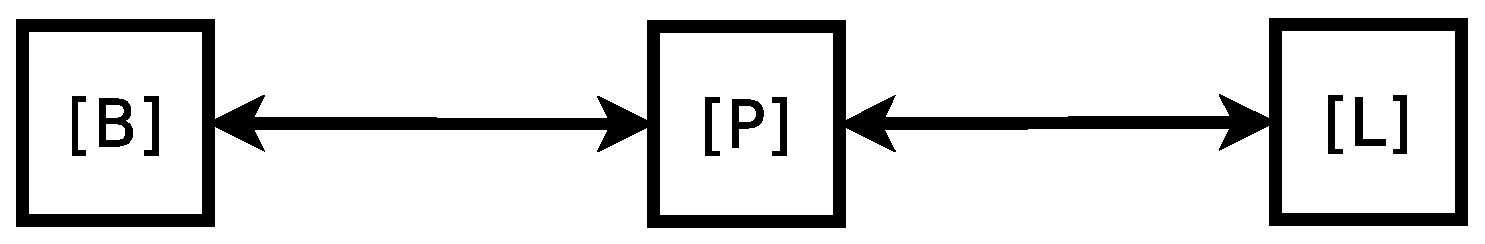
\includegraphics[width=0.48\textwidth]{archnividic.eps} & 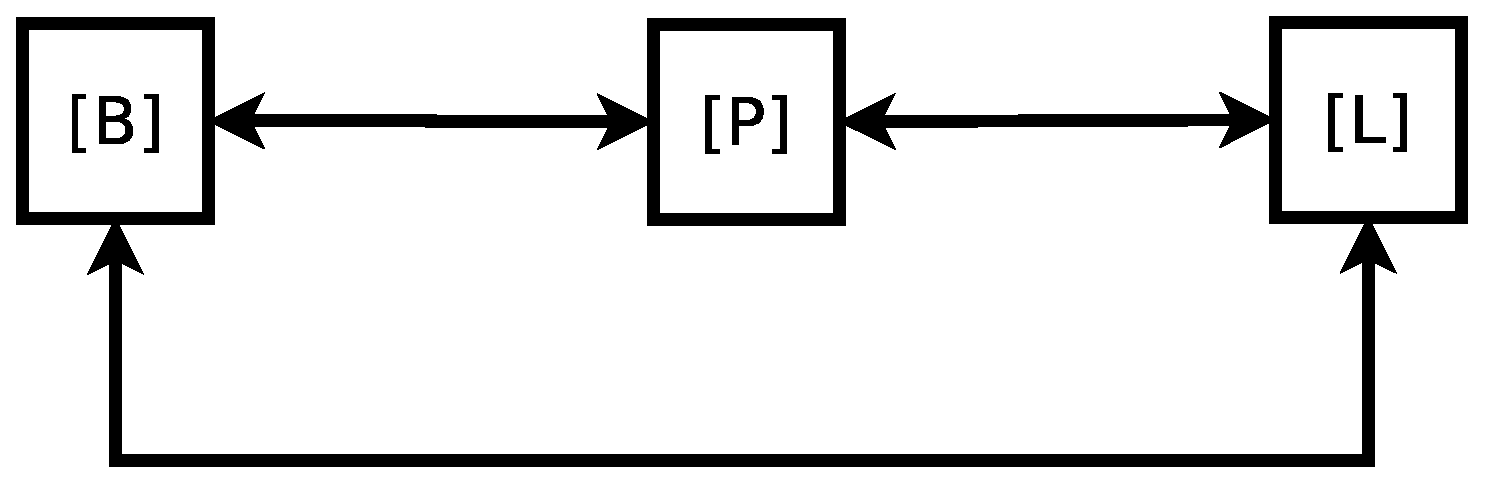
\includegraphics[width=0.48\textwidth]{archlater.eps} \\
(a) & (b)
\end{tabular}
\caption{Communication architectures, where \abbrbox{} is the \anemobox{}, \abbrphone{} is the \phone{} and \abbrlab{} is \anemolab{}. For the Nividic release (a) we assume that there is no communication link between the anemobox \abbrbox{} and the server \abbrlab{}. For later releases (b), we can imagine that such a link exists and our architecture and protocols should allow for that.}
\label{fig:arch}
\end{figure}

In order to better understand the requirements that drive the specification of the architecture and protocol, we will consider two use cases. The first use case outlines the easy case where the anemobox can talk more or less directly with the web server via the phone. The second use case is more difficult in the sense that two communication links are not available at the same time.

\subsection{Use case I: Continuous communication links}
\label{sec:easycase}
In this scenario, a sailor is on the sea with his sailboat, of the type Surprise. He has brought his mobile phone with him and the anemobox is installed on his boat. He is also sailing close to the coast and has a good internet connection to his phone. He is recording boat logs. These boat logs are continuously transferred from the anemobox to the mobile phone, and then transferred from the mobile phone to the server. After a few hours of sailing, he wants to update the calibration of his instrument, so he presses a button on his mobile phone to start calibration and a few minutes later, the calibration is done and transferred from the server to the anemobox. For the last quarter of an hour, there has been another Surprise in front of him. Thanks to a more accurate calibration, he is able to pass it eventually.

\subsection{Use case II: Discontinuous communication links}
\label{sec:hardcase}
In this scenario, a sailor is on the sea with his sailboat, sailing for a week-end. He has a mobile phone with him that is talking over bluetooth to the anemobox onboard. However, this sailor is a more modest man and he only has a prepaid phone with limited data traffic, so his phone rarely has an internet connection except when is at home connected to the WLAN. He records data on the anemobox that are transferred to the memory of the phone and saved there. When he comes home on the Sunday evening, he connects his phone to the WLAN and boat logs are uploaded to the server. Fresh calibration parameters are calculated and sent back from the server to the phone. The next week-end when he goes sailing, those parameters are transferred from the phone to the anemobox on his boat.

\subsection{Use case III: Dropping the phone in the sea}
A sailor is sailing with his boat and the anemobox on board connected via bluetooth to his phone. He is currently synchronizing the two devices but drops the phone in the sea by accident.

\section{Mailbox Model}
The mailbox model can be used to design a system that will work for all of the three use cases in the previous section. In this model, a \textbf{node} is a unit that can send and receive \textbf{packets} to other nodes. Often, a \textbf{node} can map to a physical device such as the anemobox or a mobile phone, but not always. On the server, there is one \textbf{node} for every boat with an anemobox.

In this model every node has a unique idenitification number that identifies it. It also has a set of mailboxes. Between mailboxes, messages that we call \textbf{packets} har sent. Every node has
\begin{itemize}
  \item One \textbf{mailbox of outgoing packets} for every other mailbox that it can send packets to.
  \item A \textbf{mailbox of temporary packets} that are to be forwarded to some other node.
  \item One \textbf{mailbox of incoming packets} from every other node.
  \item A \textbf{table} of the last known C-number of every sender-receiver pair.
\end{itemize}

This model is designed so that
\begin{itemize}
  \item Delivering a packet more than once is avoided (through the use of S- and C-numbers).
  \item The sender of a packet will eventually know that the packet has reached its destination.
  \item Packets will not get lost, because they are only removed once the sender knows the packet has been delivered.
  \item Timeouts and retransmission of packets is not needed. For our use cases (especially the second one), there could be delays in the order of weeks.
  \item Failure of delivering a packet should not block other packets from being delivered.
\end{itemize}

\subsection{Node synchronization}
Packets are propagated from the sending node to the receiving node through pairwise synchronizations between nodes, where they exchange information so that both nodes are up-to-date. This means that
\begin{itemize}
  \item A packet that exists on a node A, but not on a node B will result in a copy of that packet being created on node B.
  \item Sharing on information on what packets have been delivered and removal of those packets.
\end{itemize}
The protocol used for synchronizing two devices will be specified in a later document.

\subsection{Packet format}
A packet is a datastructure with these fields:
\begin{description}
  \item[Sender] The identification number of the sending node. This is the node that sends the packet. The packet will initially be put in the mailbox of outgoing packets of the sending node.
  \item[Receiver] This is the identification number of the node to which the packet is sent.
  \item[Sequence number] This is the value of a counter inside the mailbox of outgoing packets on the sending node. Whenever the the sending node sends a packet, the state of this counter is increased by one.
  \item[C-number] This is the highest sequence number among the outgoing packets on the sending node such that all packets with sequence numbers less than that number have been acknowledged. Every node in the network maintains a so called C-table that maps (sender, receiver) pairs to C-numbers. For every packet that this node receives, it will first check if the sequence number of the packet is below the C-number of (sender, receiver) the table. If yes, the packet is ignored. Otherwise, the C-table is updated if the C-number of the incoming packet is higher than the current value in the table.
  \item[Label] A code that tells what sort of data the packet carries. One special code, \texttt{acknowledged}, is reserved for packets sent back to the sender, telling them what packets can be removed.
  \item[Data] The data of the packet.
\end{description}

\subsection{Mailbox for outgoing packets}
Every node has one mailbox of outgoing packets for every receiver. The mailbox of outgoing packets can be characterized by the following fields:
\begin{description}
  \item[Receiver] This is the constant identification number of the receiver.
  \item[Sequence counter] This is a counter that holds the integer that will be put in the \textbf{Sequence number} field of the next packet to be sent.
  \item[C-counter] This is an integer of all \emph{Completed} transmissions. It means that any packet emitted from this node with a sequence number less than the C-counter has been acknowledged.
  \item[Packets] This is a list of all packets that have been emitted from this device and have sequence numbers greater or equal to that of \textbf{C-counter}. Every packet in this list has a flag which can be either \texttt{pending} or \texttt{acknowledged}. Whenever a packet with in this list with a sequence number which is the same as the C-counter is marked \texttt{acknowledged}, the C-counter is increased by one and the packet is removed from the mailbox of outgoing packets.
\end{description}

Sending a packet from the device amounts to putting the value of the \textbf{Sequence counter} in the \textbf{Sequence number} field of the packet, the value of the \textbf{C-counter} in the \textbf{C-number} field of the packet and filling all the other fields with their values. The packet is then put in \textbf{Packets} of the outgoing mailbox and the \textbf{Sequence counter} is increased by one. Whenever the node is synchronized with another node, this packet and possibly other packets too, will be copied to that node.

\subsection{Mailbox for temporary packets}
This is a mailbox of packets where the current node is neither the sender nor the receiver: It only keeps the packets so that they can be forwarded on the next synchronization. It is important to note that it will only accept packets with sequence numbers greater or equal to the corresponding C-number looked up in the C-table. Also, whenever the C-table is updated, all packets in with sequence numbers that are less than their corresponding C-numbers in the C-table are removed.

\subsection{Mailbox of incoming packets}
A node has one mailbox of incoming packets for every other node from which it could receive packets. It will only accept packets with a sequence number greater or equal to the corresponding C-number in the C-table, thereby avoiding double delivery. Also, whenever the C-table is updated, packets in the incoming mailbox with sequence numbers less than their corresponding C-number in that table can be safely removed. 

For every $n$ packets received (in any order), an acknowledgement packet is sent back to the sender listing the sequence numbers of those $n$ packets so that the sender can mark those packets as acknowledged. The acknowledgement packet is like any other packet with the only exception that its \textbf{Label} field is set to \texttt{acknowledged}.

\subsection{C-table}
The C-table maps (sender, receiver) identity pairs to C-numbers. The purpose of the C-table is to provide a mechanism for removing packets that have been delivered in order to save space on all devices. It has two functions:
\begin{itemize}
  \item It can be used by the node to see what packets that it is already storing, can be removed.
  \item It can be used to ignore incoming packets that are outdated.
\end{itemize}
Whenever the node sees a packet, it will form a (sender, receiver)-pair from that packet and look up the C-number in the table. If the sequence number of the packet is less than the C-number, the packet is outdated and can be ignored. Otherwise, if the C-number of the packet is greater than the C-number in the table, the C-number in the table will be updated to the C-number in the packet.

\subsection{Sequence number generation}
A sequence number is obtained from the sequence counter in the outgoing mailbox of the sending device. This counter is initialized to 0. All packets and mailboxes should allow for sufficiently high sequence numbers that can possibly be generated throughout the lifetime of the Nividic product. From an implementation point of view, it would make sense to allow for arbitrarily high integers to completely eliminate the risk that the space of numbers is exhausted.

\subsection{Similarities and differences with the TCP protocol}
The protocol used for delivering packets is inspired by the TCP protocol in the sense that a concept similar to sequence numbers is used. However, it is different in order to accomodate for the various use cases where it is to be used. For instance, in use case II explained in section \ref{sec:hardcase}, a three-way handshake mechanism of the TCP protocol in order to synchronize sequence numbers would take a week to complete. Therefore, something different is necessary.

Another difference is that every intermediate node used to deliver a packet will keep the packet until it knows it has been delivered and can be reliably removed. Whenever two nodes are connected, their mailboxes will synchronize their data eagerly so that the packets are replicated on both nodes. This is in contrast to the TCP protocol, where the intermediate nodes just forward the packets. In the TCP protocol, a the sender of a packet who does not receive an acknowledgement within a certain time since it sent its packet, will retransmit it. A timeout in our scenario, however, would be probably not be very useful because even a month could be a perfectly reasonable time until an acknowledgement would be returned to the sender, depending on what sort of connection to the internet the sailor has.

\section{Discussion}
In order to optimize the delivery of packets and reduce unnecessary transmissions of data, domain-specific constraints may be introduced so that certain packets only can synchronize in one direction for certain node pairs. For instance, if the a mobile phone needs to send packets to the server anemolab, it would probably not be useful to send those packets also to the anemobox, especially not if the anemobox does not have an internet connection.

We also discuss some other design decisions, especially related to mailboxes.

\subsection{Why have one mailbox of outgoing packets for \emph{every} receiver instead of one common mailbox of outgoing packets for all receivers?}
This has to do with the C-counter. The C-counter will be increased by one whenever a sent packet with the sequence number of the C-counter is acknowledged. Suppose that a packet is sent to a device and that device is dropped in the sea. This packet will never be marked as acknowledged and the C-counter will be stuck forever, meaning that packets will accumulate on all devices as they are sent. If we have separate outgoing mailboxes and every such mailbox has its own C-counter, the C-counters of devices that were \emph{not} dropped in the sea can still be increased and packets can be removed, preventing accumulation of packets as the system is being used.

\subsection{Why have one mailbox of incoming packets for \emph{every} sender, instead of one common mailbox of incoming packets for all senders?}
This has to do with the acknowledgement. If we send an acknowledgement packet for every $n$ packets received, those packets could all have different senders, and we would have to send that packet to all senders. Seperarating the incoming packets into seperate mailboxes should be more efficient, since for every $n$ packets we receive to such a mailbox, we only need to send one acknowledgement packet to the single sender of those packets.

\subsection{Protocol for synchronization}
We outline in a separate document the details about the protocol used for synchronizing two nodes and their mailboxes. This protocol will specify how to nodes talk with each other in order to synchronize.
\end{document}

